\pref{def:PH} introduces the Process Hitting~(PH)~\cite{PMR10-TCSB}
which allows to model a finite number of local levels,
called \emph{processes},
grouped into a finite set of components, called \emph{sorts}.
A process is noted $a_i$, where $a$ is the sort's name,
and $i$ is the process identifier within sort $a$.
At any time, exactly one process of each sort is \emph{active},
and the set of active processes is called a \emph{state}.

The concurrent interactions between processes are defined by a set of \emph{actions}.
Each action is responsible for the replacement of one process by another of the same sort
conditioned by the presence of a set of other processes in the current state.
An action is denoted by $\PHfrappe{A}{b_j}{b_k}$, which is read as "all the processes in $A$ cooperate to \emph{hit} $b_j$ and make it \emph{bounce} to $b_k$'',
where $A$ is a set of processes (with at most one process per sort) and
$b_j$, $b_k$ are processes of sorts $b$.
We call $A$, $b_j$ and $b_k$ respectively the set of \emph{hitters}, the \emph{target} and the \emph{bounce} of the action.
We also call a \emph{self-hit} the special case of actions with exactly one hitter which is equal to the bounce of the action, that is, of the form:
$\PHfrappe{b_j}{b_j}{b_k}$.

The PH is therefore a restriction of Synchronous Automata Networks where each transition
changes the local state of exactly one automaton,
therefore restricted to an asynchronous framework,
as explained below.
This restriction on the actions was originally more strict and chosen to permit
the development of efficient static analysis methods
based on abstract interpretation~\cite{PMR12-MSCS}.

\begin{definition}[Process Hitting]\label{def:PH}
  A \emph{Process Hitting} is a triple $(\PHs,\PHl,\PHa)$ where:
  \begin{itemize}
    \item  $\PHs = \{a,b,\dots\}$ is the finite set of \emph{sorts};
    \item  $\PHl = \prod_{a\in\PHs} \PHl_a$ is the set of \emph{states} where
      $\PHl_a = \{a_0,\dots,a_{l_a}\}$
      is the finite set of \emph{processes} of sort $a\in\Sigma$
      and $l_a$ is a positive integer, with $a\neq b\Rightarrow \PHl_a \cap \PHl_b = \emptyset$;
    \item $\PHa = \{ \PHfrappe{A}{b_j}{b_k} \mid A \in \PHl^{\diamond} \wedge b \in \PHs \wedge b_j \neq b_k \wedge \PHl_b \cap A \neq \emptyset \Rightarrow A=b_j\}$ is the finite set of \emph{actions},
    with $\PHl^{\diamond}$ the set of all the sub-states of $\PHl$
    (that is, containing at most one process from each sort).
      %$\PHa$ = \{ $\PHfrappe{A}{b_j}{b_k}$ with $A \in \PHl^{\diamond} \wedge b \in \PHs \wedge b_j \neq b_k \wedge$ if $b_j \in A \Rightarrow A=b_j$ \}.With $\PHl^{\diamond}$ the set of all the sub-states of $\PHl$. 
  \end{itemize}
\end{definition}

\begin{example}
\pref{fig:ph} represents a PH model with five sorts ($a$, $b$, $c$, $d$ and $e$) and four actions among which one is a self-hit ($\PHfrappe{d_1}{d_1}{d_0}$).
\begin{figure}[t]
  \centering
  \scalebox{1.3}{
  \begin{tikzpicture}[apdotsimple/.style={apdot}]

   \TSort{(3.5,0.5)}{a}{2}{r}
    \TSort{(3,4.5)}{b}{3}{t}
    \TSort{(7,1)}{e}{2}{r}  
    \TSort{(0,3)}{c}{2}{r}
    \TSort{(0.5,0)}{d}{2}{r}
    
    \THit{d_1}{selfhit}{d_1}{.north west}{d_0}
       
   % \THit{e_1}{selfhit}{e_1}{.north east}{e_2}
% b en 3 niveaux avec un selfhit de 1 à 2
   \THit{d_0}{}{a_0}{.west}{a_1}
   \TActionPlur{a_1, b_1}{e_0.north west}{e_1.west}{}{5.5,2.5}{left}
   \TActionPlur{a_1, c_1}{b_0.south}{b_1.south west}{}{2,3}{right}

    \path[bounce, bend right]
      % \TBounce{d_1}{}{d_0}{.north}
   \TBounce{d_1}{}{d_0}{.north west}
  %    \TBounce{e_1}{}{e_2}{.north east}
    ;
   \path[bounce, bend left]
   \TBounce{a_0}{}{a_1}{.south west}
%	\TBounce{z_0}{bend left=90}{z_1}{.south east}
    ;
    \TState{a_0, b_0, c_1, d_1, e_0}
  \end{tikzpicture}
  }
  \caption{\label{fig:ph}
An example of PH model with five sorts: $a$, $b$, $c$, $d$ and $e$. Boxes represent the sorts (the biological components), circles represent the processes (the component levels), and the actions that model the dynamic behavior are depicted by pairs of arrows in solid and dotted lines. $a$, $d$, $c$ and $e$ are all either at level $0$ or $1$, and the sort $b$ has $3$ levels ($0$, $1$, $2$). The grayed processes stand for a possible initial state $\PHstate{a_0, b_0, c_1, d_1, e_0}$.
\Maxime{Plutôt que cet exemple, pourquoi ne pas mettre le PH qui donne le graphe de la Figure 2 ?}
  }
\end{figure}

\end{example}

A \emph{state} of the network is a set of active processes containing exactly one process of each sort.
The active process of a given sort $a \in \PHs$ in a state $\PHst \in \PHl$
is noted $\PHget{\PHst}{a}$.
For any given process $a_i$ we also note: $a_i \in \PHst$ if and only if $\PHget{\PHst}{a} = a_i$; it means that the biological component $a$ is in the condition labeled $i$ within state $\PHst$.

\subsection{Attractors in Process Hitting}

The study of the dynamics of biological networks was the focus of many works, explaining the diversity of network modelings and the different methods developed in order to identify attractors \cite{skodawessely2011finding, zhang2007algorithms, mushthofa2014asp, akutsu2012finding, berntenis2013detection}.
In this paper we focus on several sub-problems related to this: we seek to identify the steady states, the cycles and the attractors. %Then we verify the reachability of these attractors. \\
In the following, we consider a BRN modeled in PH $\PH=(\PHs,\PHl,\PHa)$,
and we formally define these properties.
We note that because PH encompasses Thomas modeling, all our results are also applicable to this formalism, as well as any other framework that can be described with PH.
%How to verify them with the help of ASP is the subject of the rest of this paper.
%and explain how they could be verified on a such network.

In \pref{def:playableAction} we formalize the dynamics of a PH which is based on the actions in an asynchronous fashion.
An action can be played in a given state if all of its hitters and its target are active in this state; playing this action then means replacing the target process by the bounce process.
Thus, the set of playable actions in a given PH state gives the set of transitions starting from this state in the state-transition graph.
As a consequence, the playability of an action only depends on the current state;
furthermore, the dynamic evolutions of the model are purely non-deterministic
because several branchings can be potentially chosen between at any step.

\begin{definition}[Playable action \& Successor]
\label{def:playableAction}
Let $\PH = (\PHs,\PHl,\PHa)$ be a Process Hitting, $\PHst \in \PHl$ a state and $h = \PHfrappe{A}{b_j}{b_k} \in \PHa$ an action of this model.

We say that the action $h$
is \emph{playable in state~$\PHst$} if and only if
$A \subseteq \PHst$ and $b_j \in \PHst$ (\ie $\forall a_i \in A$, $\PHget{\PHst}{a} = a_i$ and $\PHget{\PHst}{b}=b_j$).

The resulting state after playing this action $h$ in $\PHst$
is called a \emph{successor} of $\PHst$ and
is denoted by $(\PHst \play h)$,
where $\PHget{(\PHst \play h)}{b} = b_k$ and
$\forall c \in \PHs, c \neq b \Rightarrow \PHget{(\PHst \play h)}{c}=\PHget{\PHst}{c}$.
\end{definition}

Since we are considering only the asynchronous updating scheme (\Emna{ref asynchrone}), only one component can change its expression level from a state to any of its successors (\ie only one action is played at each step). In the following, if $\PHst \in \PHl$ is a state,
we call \emph{scenario from~$\PHst$}
any sequence of successive states from $\PHst$
obtained by playing some actions successively,
and we denote $\Sce(\PHst)$ the set of all scenarios from $\PHst$.

\begin{example}
In the PH model example of \pref{fig:ph}, let us consider an initial state $\PHst_0 = \PHstate{a_0, b_0, c_1, d_1, e_0}$ ---~or, knowing the sorts order, $\PHst_0 = (0, 0, 1, 1, 0)$. The only possible and longest sequence of successive states from $\PHst_0$ is the following:
  \[(0, 0, 1, 1,0) \rightarrowtail (0, 0, 1, \underline{0}, 0) \rightarrowtail (\underline{1}, 0, 1, 0, 0) \rightarrowtail (1, \underline{1}, 1, 0, 0) \rightarrowtail (1, 1, 1, 0, \underline{1}).\]
Therefore, the set $\Sce(\PHst_0)$ contains five elements: all sub-sequences consisting of the beginning of this one.
\Maxime{Reformuler}
\end{example}

A \emph{fixed point}, also called \emph{steady state},
is a state which has no successor,
as given in \pref{def:fixpoint}.
Such states have a particular interest as they denote states in which the model
stays indefinitely,
and the existence of several of these states denotes a switch in the dynamics~\cite{wuensche1998genomic}.

\begin{definition}[Fixed point]
\label{def:fixpoint}
  A state $\PHst \in \PHl$ is called a \emph{fixed point}
  (or equivalently \emph{steady state})
  if and only if it has no successors.
  In other words, $\PHst$ is a fixed point if and only if no action is playable in this state:
$$ \forall \PHfrappe{A}{b_j}{b_k} \in \PHa, A \not\subseteq \PHst \vee b_j \notin s \enspace. $$
\end{definition}

A finer and more general dynamical property consists in
the notion of \emph{attractor}.
Such a structure, formally described in \pref{def:attractor},
is a minimal set of states in which the system loops indefinitely (see \pref{fig:transition-graph}).
In fact, this is equivalent to say that an attractor is a connected set of states: from each state, all other states can be (indirectly) reached.
This definition permits us to define an attractor by using the notion of a \emph{cycle},
which we define as a set of states where each state can loop on itself.

%states that starting from a given initial state, it is possible
%to reach a given goal, that is, a state that contains a process
%or a set of processes.
%Checking such a dynamical property is considered difficult
%as, in usual model-checking techniques,
%it is required to build (a part of) the state graph,
%which has an exponential complexity.

\begin{definition}[Cycle \& Attractor]
\label{def:cycle}
\label{def:attractor}
%A set of states $\mathbf{C} = \bigcup\limits_{i=1}^{N} \PHst_{i}$
A set of states $\mathbf{C} = \{ \PHst_{i} \}_{i \in \segm{1}{N}}$
is called a \emph{cycle} of size $N$ if and only if $\forall \PHst \in \mathbf{C}, \PHst \in \Sce(\PHst)$.
\Maxime{ATTENTION : il y a une confusion entre scénario et ensemble des états accessibles ici ! Il faut soit refaire la def de $\Sce$, soit rajouter une def pour les états accessibles.}

%A set of $N$ states $\Delta = \bigcup\limits_{i=1}^{N} \PHst_{i}$
A set of $N$ states $\Delta = \{ \PHst_{i} \}_{i \in \segm{1}{N}}$
is called an \emph{attractor} of size $N$ if and only if $\Delta$ is a cycle and $\forall h \in \PHa $ playable in $\PHst \in \Delta$, $(\PHst \play h) \in \Delta$.
\end{definition}

\Emna{du contenue à propos les cycles}

By definition, if the system evolves and reaches any state of an attractor, it will infinitely cycle into the states of this same attractor.
On the other hand, we also note that every maximal scenario of a network eventually converges to either a fixed point or an attractor, both of which cannot be escaped.
Therefore, we can also identify a fixed point (\ie steady state) with an attractor of size~1.

\begin{figure}[t]
   \caption{\label{fig:transition-graph} A state transition graph of a PH model with 3 sorts (one sort with two levels $0$ or $1$ and two other sorts have three levels $0$, $1$ and $2$). This graph contains two attractors (size 2 and size 4) and one fixed point}
   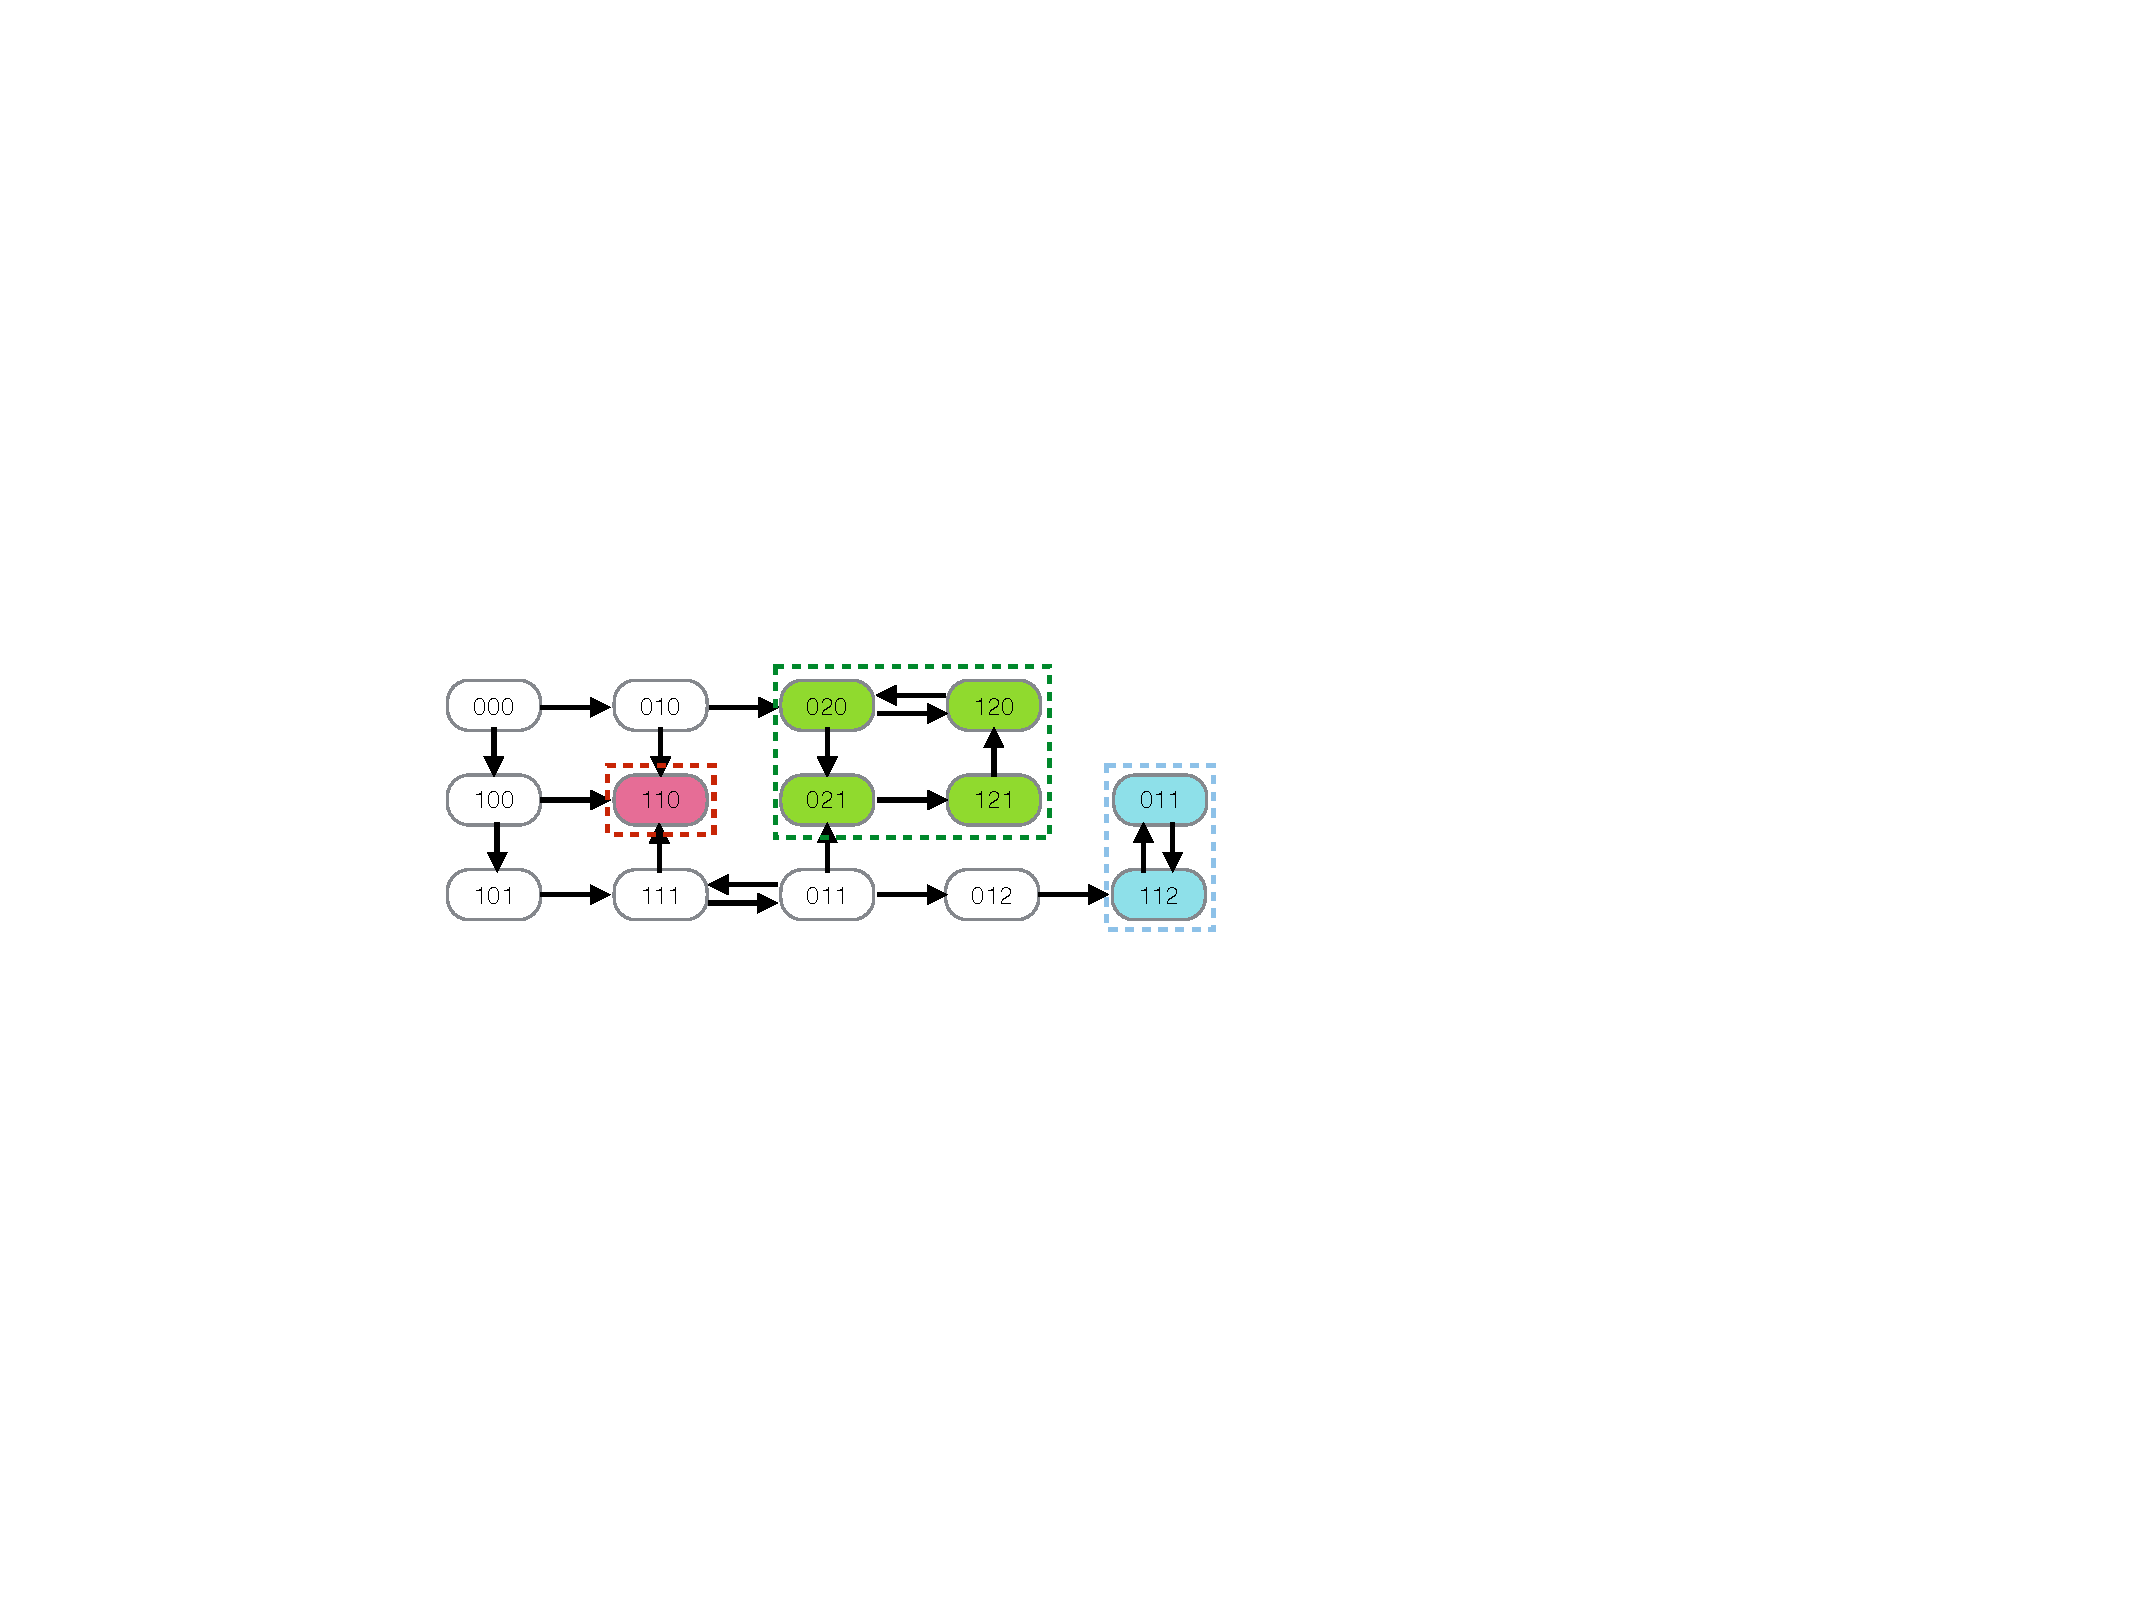
\includegraphics{figures/transition-graph.pdf}
\end{figure}

\medskip
The aim of the rest of this paper is to tackle the enumeration of fixed points (\pref{sec:fixpoint}) and attractors (\pref{sec:attractors}) in a PH model.
For this, we use Answer Set Programming (ASP), which is a declarative paradigm dedicated to the resolution of complex problems. ASP is presented in the next section.
